\chapter{Experimental Setup}
In this chapter we will look at the equipment we use in our recordings.
Further we will go into detail about the limitations and possibilities introduced by this setup, and discuss alternative approaches.

\label{chp:experimental_setup} 

\section{Microphone selection}\label{sec:ch3_microphone_selection}

We want to do frequency spectrum analysis on the recordings, hence we are limited by the Nyquist frequency, given by \autoref{eq:nyquist_frequency}.
Our initial setup uses a Knowles Ultrasonic microphone, connected to a National Instruments myDAQ. 
This this setup we reach are able to record with a sampling rate \({F_{s}}\) of \(200\)kHz. 
By \autoref{eq:nyquist_frequency} we then find that our maximum frequency for spectrum analysis is \(100\)kHz.
The original paper \todo{cite} suggests that we should be be able to observe distinctions between CPU operations in far lower than this, so we should be able to achieve interesting results using this simple setup.

\begin{equation}\label{eq:nyquist_frequency}
F_{nc} = \frac{F_{s}}{2}
\end{equation}

There are interesting implications of this setup; the the microphone itself is very small as well as being very cheap, costing only a few dollars\cite{butikken}. 
Hence, this is a very portable setup, that can be hidden and used in covert operations against unsuspecting targets, in for instance a side channel attack against a vulnerable RSA implementation, as suggested in \cite{paper}.
The low cost of the parts used, less the myDAQ, also makes it disposable.
A small microphone also enables the possibility to hide the whole setup inside the casing of a desktop computer or a server, thus possibly making side channel attacks easier due to a better signal-to-noise ration due to the reduced distance between the source and the microphone.

\subsection{Knowles Ultrasonic SPU0410LR5H Configuration}\label{sec:ch3_knowles_configuration}

\begin{wrapfigure}{r}{0.5\textwidth}
    \vspace{-20pt}
    \centering
    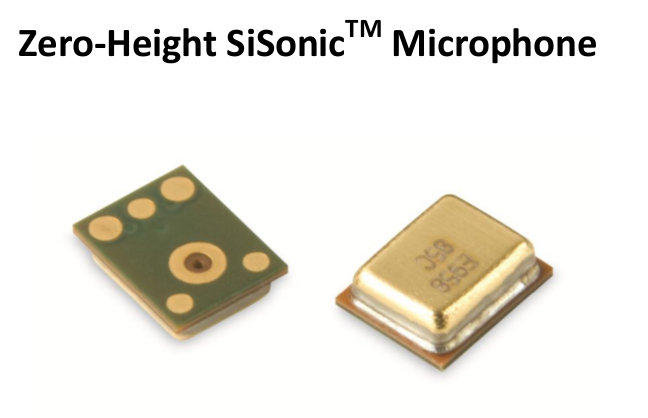
\includegraphics[scale=0.3]{knowles_microphone.png}
    \vspace{-20pt}
    \caption{Knowles Ultrasonic SPU0410LR5H~\cite{url:knowles_spec}}
    \vspace{-20pt}
    \label{fig:knowles_microphone}
\end{wrapfigure}

The Knowles Ultrasonic SPU0410LR5H microphone in \autoref{fig:knowles_microphone} is able to detect sound at least up to 80kHz with a -4dB sensitivity\cite{url:knowles_spec}.
To be able to record frequencies up to 100kHz, we need the National Instuments (NI) myDAQ~\cite{url:NI_myDAQ} to sample the sound at a sampling frequency \(F_{s}\) of 200kHz.
The microphone is connected to a 4.5V battery and directly in to Analog Input 0 on the myDAQ device. 

The myDAQ device has a built in an amplifier (OPA1642) seen in the hardware block diagram at page 4 in the myDAQ user guide~\cite{url:NI_myDAQ_userguide}. 
The OPA1642 has a gain of 60 dB at 10kHz and 40 dB at 100kHz seen in figure 5 at page 5 in the OPA1642 specification~\cite{url:TI_opa1642}.
With an input voltage of +-10mV, the nominal output is +-1V as illustrated in \autoref{fig:op_amp_illustration}
\todo{check this with Tim Cat Netland}

\begin{figure}[h]
  \begin{circuitikz} 
    \draw 
    (0,0) node[op amp] (opamp1) {}
    (opamp1.+) node[left ] {10mV @100kHz $v_+$}
    (opamp1.-) node[left ] {$v_-$}(1,0)
    (1,0) to[voltmeter, l=1<\volt>] (4,0);
  \end{circuitikz}
  \caption{Op Amp illustration}
  \label{fig:op_amp_illustration}
\end{figure}


\subsection{Brüel\&Kjær 4191 Configuration}\label{sec:ch3_bruel_kjaer_configuration}

Much like one of the lab setups~\ref{sec:lab_setup} from the original paper we use a Brüel\&Kjær 4191 microphone that is able to do precise measurements up to frequencies around 40kHz~\cite{url:bk4191_spec}.
The microphone is then connected to a preamplifier \todo{write about the preamp we used in the experiment} which is then connected to a Brüel\&Kjær 5935 microphone power supply and amplifier.
The output signal is then led into the NI myDAQ and further in to our computer, i.e. the adversary in this case.


\section{Processing and signal extraction}\label{sec:ch3_processing_signal_extraction}

The captured sound is stored in a WAV file.
This file is processed in our self written software, which utilizes libraries such as FFTW \cite{url:fftw} and libsndfile \cite{url:libsndfile}.
The samples are divided into windows \( W \), where \( \lvert W \rvert = 2^{n} \) where \( n \) is a non-zero positive integer.

The WAV file contains a mono signal. In the WAV format, frames representing each sample is stored subsequently, such that the sample \( s_{f,c} \) represents the \gls{PCM} response for frame \( f \) channel \( c \). 
For a stereo signal this means that \( f \in \left [ 1, 2 \right ]  \), and thus the samples are ordered  \( s_{0,0}, s_{0,1}, s_{1,0}, s_{1,1}, ... , s_{n,0}, s_{n,1} \). 
Since we want to work on a mono signal, we simply ignore all frames where \( f \neq 0 \), which with our setup means that we use all samples in the stored file.

The captured sound file is Fourier transformed using a window size of 4096 samples, and the hamming window function. The resulting power spectra are studied, with emphasis on how they are evolving in the time domain, and how they correlate to the expected effects of the software described in \autoref{chp:predictable_execution}

\section{Capturing audio fingerprint}\label{sec:ch3_capturing_audio_fingerprint}

Our guess, based on the original paper~\cite{DBLP:conf/crypto/GenkinST14}, is that the sound derives much likely from some coil whine around the CPU. 
Therefore we are positioning the microphones as close to the CPU as possible. 
When listening to the Lenovo T60p, we unmounted the keyboard letting us position the microphone on top of the cooling element for the CPU as illustrated in figure~\ref{fig:T60p_knowles_position}. 

% \begin{wrapfigure}{r}{0.5\textwidth}
%     \vspace{-20pt}
%     \centering
%     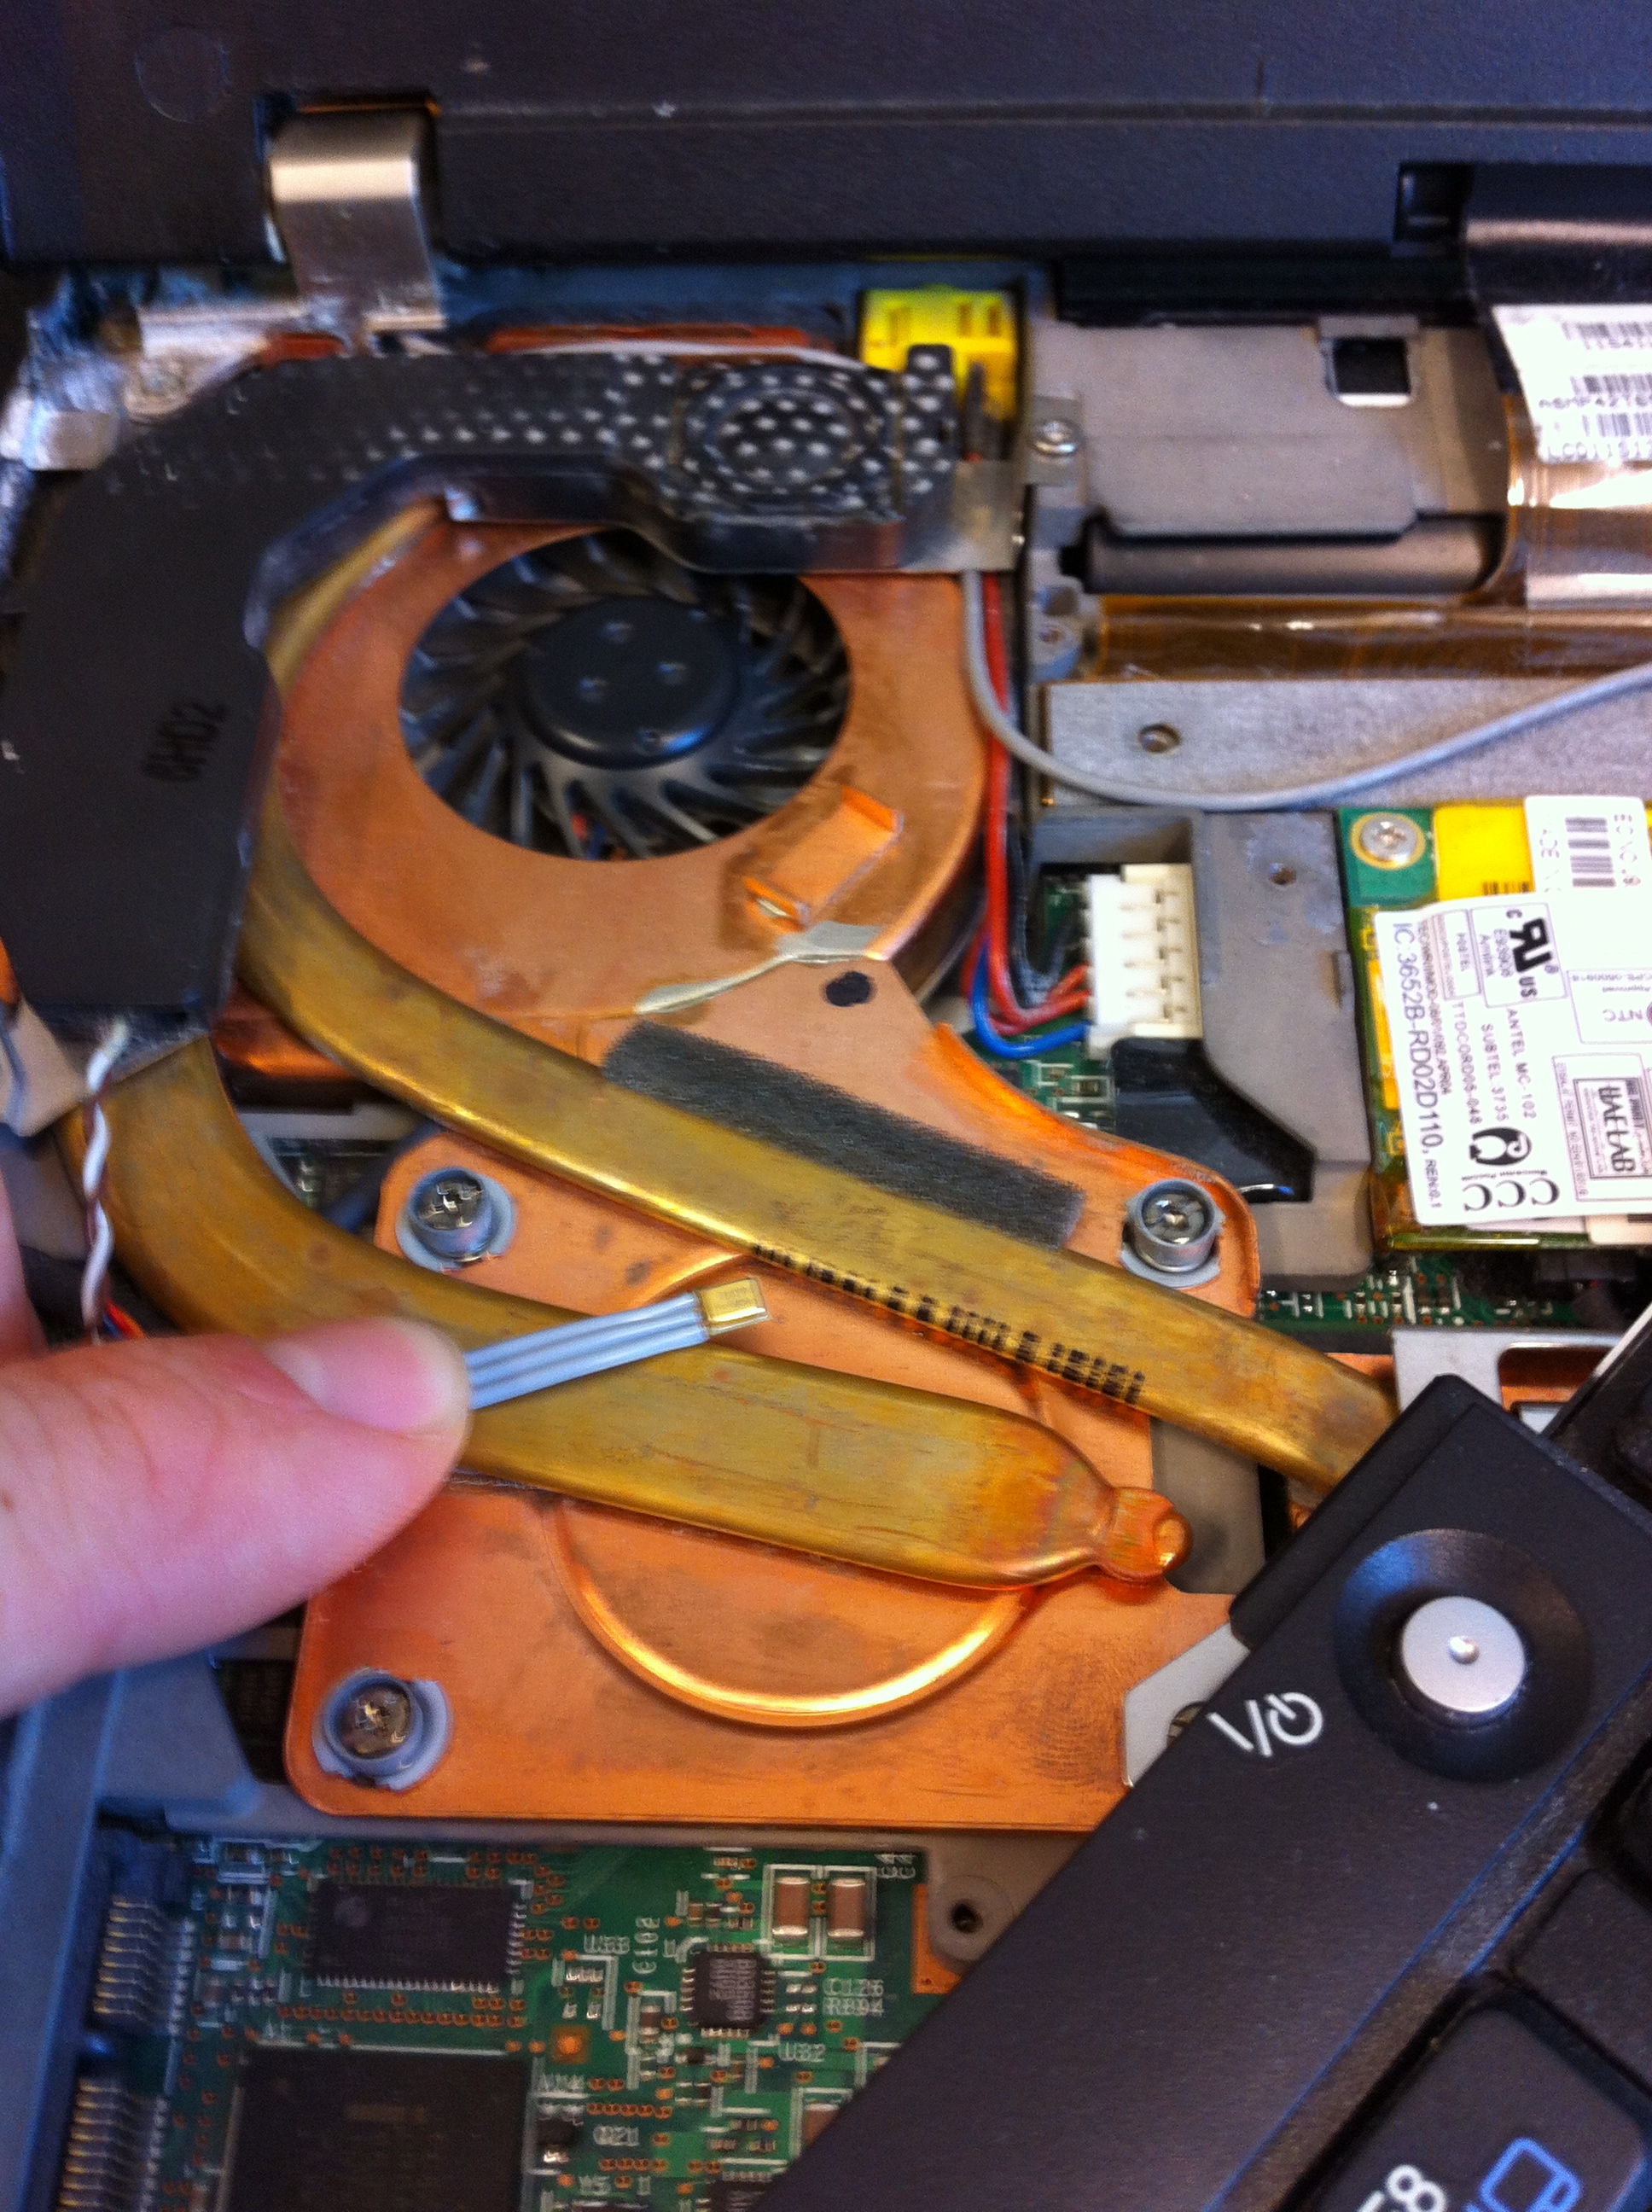
\includegraphics[width=2in]{T60p_knowles_position.JPG}
%     \vspace{-20pt}
%     \caption{The Knowles Ultrasonic SPU0410LR5H~\cite{knowles_spec} microphone position when recording close to the CPU on the Lenovo T60p.}
%     \vspace{-20pt}
%     \label{fig:T60p_knowles_position}
% \end{wrapfigure}


\section{Experimental plan}\label{sec:ch3_experimental_plan}\todo{Put this in appendix}

Our experimental plan consists of different test cases on different subjects with different microphone setups. 
Each test case is performed with all microphone setups and with all test subjects. 

To calibrate each microphone, we are using a tweeter to play a sinus wave from a tone generator. 
The frequencies that will be generated are 10kHz, 20kHz, 30kHz and 40kHz.
After calibration, we will record the ambient noise where we are doing the experiment.
This is to eliminate other sources of noise when we are doing the experiments.
We will also do the experiments in an anechoic chamber, which will eliminate close to all other sound sources.

\subsection{Test cases}


\begin{enumerate}
  \item[CPU idle] Record when the CPU is idle. 
  We are doing this to find out what the CPU possibly might leak when doing nothing. 
  Then we perform a CPU load, micro instructions and finally decryptions.
  \item[CPU load] Exposing the CPU from low to high load.
  Read more about how we do the CPU load in chapter~\ref{chp:analyzing}.
  \item[Micro instructions] Read more about how we do the micro instructions in chapter~\ref{chp:analyzing}.
  \item[Decryption] As stated in the original paper, we should be able to detect when the CPU is doing a RSA decryption. 
  For this we decrypt an encrypted file with a RSA 4096-bit key using GnuPG v1.4.15~\cite{url:GnuPG_1.4.15}
\end{enumerate}

\subsection{Test subjects}
On all test subjects, we are planning to record as close as possible to the CPU. 
The following devices is tested:

\begin{itemize}[topsep=-1em,parsep=0em,itemsep=0em]
 \item Lenovo T60p
 \item Raspberry PI
 \item Dell Latitude D430
 \item Dell Latitude D400
\end{itemize}

\subsection{Microphones}
The microphones we use during our experments:
>>>>>>> ref: fixed references, chp4: added info about decryption

